\documentclass[12pt]{article}

\usepackage[utf8]{inputenc}
\usepackage{colortbl}
\usepackage{float}
\usepackage{graphicx}

\definecolor{gray}{rgb}{0.4,0.4,0.5}
\date{24 de Agosto de 2019}

\title{\vspace{-3.0cm}Lista 1 de exercícios - MAC0344}
\begin{document}
	\maketitle
	\noindent\textbf{E1.} O Brasil tem atualmente 3 supercomputadores na lista top500.\\
	São eles, seguidos de suas informações:\\
	\begin{table}[H]
		\begin{tabular}{|l|l|l|l|l|l|} \hline 
			Nome  & Colocação &Local & \#Cores & Linpack [TF/s] & Vel. Max [TF/s]\\ \hline
			Fênix & 142 & Petrobras (RJ) & 48,384 & 1,836 &  4,297.421\\ \hline
			BC1	  & 419 & ? & 38,400 & 1,123.15 & 1,413.12 \\ \hline
			BC2	  & 429 & ? & 38,400 & 1,123.15 & 1,413.12 \\ \hline
		\end{tabular} \vline 
	\end{table} 
	\noindent\textbf{E2.}\\
	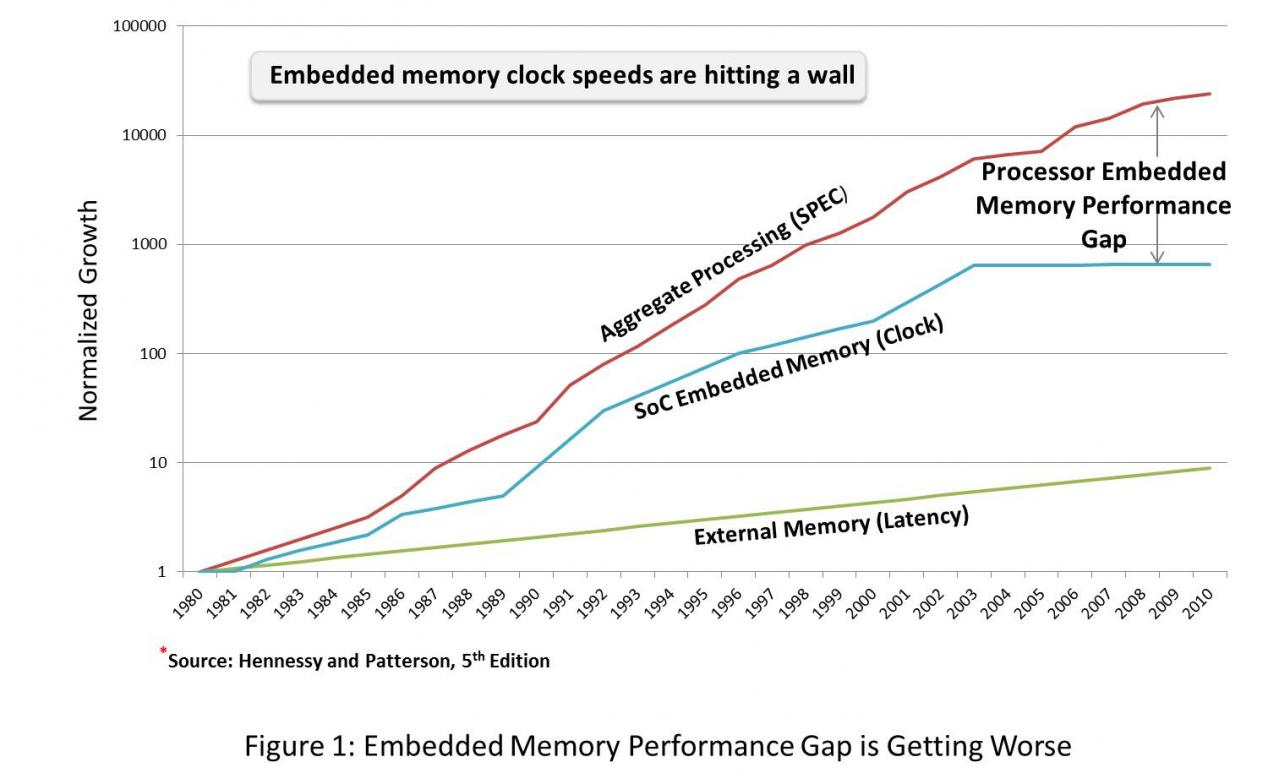
\includegraphics[height=6cm]{graph-01} \\
	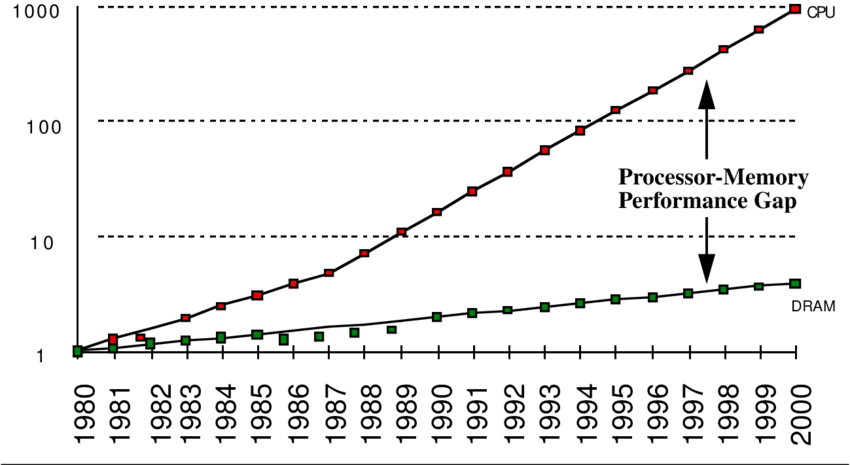
\includegraphics[height=5.5cm]{graph-02} \\
	Como podemos observar, a velocidade do processador cresce mais do que a velocidade da memória. \\\\
	
	Gráfico 1 – https://semiwiki.com/semiconductor-ip/1448-mind-the-gap-overcoming-the-processor-memory-performance-gap-to-unlock-soc-performance/, acessado 23/08/2019 \\
	
	Gráfico 2 –  https://www.researchgate.net/figure/Processor-Memory-Performance-GapHen96\_fig1\_3214931, acessado 23/08/2019
	
\end{document}